\chapter{Introduction}

Provenance as a concept has been around for a long time. It originally comes from the Latin word \textit{provenio}, meaning ``to come forth'' and its primary use has been in the field of art and antiques where provenance is used to identify the authenticity and quality of a piece of artwork. For anyone with a background in databases this term may also be familiar as the concept of linking tuples from the output of a query to the reason they exist.

In this paper the provenance we refer to is that of \textit{digital provenance}. It is a type of metadata representing the lineage of an object. Naively it can be compared to the information stored in revision history systems like that used in google docs\footnote{Google docs: \url{https://docs.google.com}} or version control
% TODO: git and mercurial links
systems such as git\footnote{GIT\: \url{}} or mercurial. These systems are usually limited to storing revisions and authorship. Provenance extends beyond this by making it possible to store and ultimately trace what other entities and activities led to a digital objects current state. By studying the provenance of a file or digital object a user is able to identify what processes, other files and bits of data influenced the file.

Provenance has the potential for usefulness in many different fields. The foremost and focus of this paper is the field of personal data management, allowing users to understand how their data is used. Often when a user chooses to share their personal data it is aggregated, anonymised or passed through any number of functions. By exploring provenance users have the ability to understand exactly how much and in what state their personal data is used.

An example to illustrate this point. Alice has a report that describes her current fitness level as well as outlining possible improvements. Viewing the provenance of
% TODO: Fitbit and Withings footnotes
this report shows which sources have been used (e.g. Fit-Bit data to track steps, Withings scale to track weight) and what processes analysed them. In this case it could show that Alice's fitness report was generated using step data from her FitBit data, passed through a summarisation process that summarises 15 minute interval data into daily steps. The provenance of her fitness report can be traced backwards to find this information, it is also possible to trace information forward, possibly in the case of errors in data. Alice remembers that she lent her FitBit to a friend to try for a week, causing errors in her data, in this case she would want to trace the erroneous information forward to see what other processes and entities it effected and would need to be corrected.

Provenance has the potential to be useful in any field where the lineage of an object needs to be stored. One example would be in data warehouse systems where information about data transformations and data origins is stored. Research into storing provenance in
% TODO: reference to block chains
block-chains or similar systems has been undertaken as it would prevent meddling of historical information, something that could be useful in high risk environments such as accounting and banking.

Early provenance systems stored provenance information in a variety of different flat
% TODO: prov reference
file formats. Since 2013, the PROV specification has provided a generic model for storing provenance with a number of serialisations (PROV-N, XML, JSON and RDF). PROV identifies provenance elements as three main concepts:

\begin{itemize}
	\item Entities: Physical, digital, conceptual objects
	\item Activities: Elements that cause an entity to come into existence
	\item Agents: Someone or something that can be assigned responsibility for an activity taking place.
\end{itemize}

The industry standard for representing these concepts is on an acyclic graph. An example of this with each of the three main concepts can be see in Figure~\ref{fig:key-concepts}.

\begin{wrapfigure}{r}{0.5\textwidth}
	\centering
	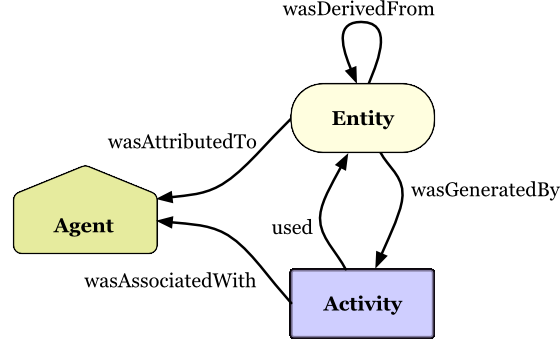
\includegraphics[width=\linewidth]{key-concepts}
	\caption{Key Concepts and relationships from the PROV standard displayed in a labelled acyclic graph.}
	\label{fig:key-concepts}
\end{wrapfigure}

Provenance can be stored in a variety of different granularity's and levels. The three main levels of capture are system-level, application-level and network level. System level provenance is the lowest level and will often capture operating system activities such as which application ran when to effect a piece of data. Application level provenance is usually limited to a single application, and will often capture information directly related to the user using that application. Network provenance often captures information via network attached devices and stores lineage originating from multiple machines. These three levels are quire broad and do not cover all use cases but they do give a good point for starting discussion and comparing provenance capture tools.

Provenance is also captured at different levels of granularity. Using the example of Alice as above, a system may capture information about her step data at the smallest granularity: how many steps every 15 minutes, or it may store the information at a larger granularity: daily step data.

As seen in Figure~\ref{fig:key-concepts} provenance graphs are most often represented as directed acyclic graphs
% TODO: Novel provenance representation citing
(although there has been some other novel approaches). A problem that quickly occurs is that provenance can become incredibly large, particularly in the case of OS level recording as it is usually at a low granularity where a lot of data is recorded in a small amount time. Because provenance is inherently historical it is forever growing in size (as of yet there's no standard for going back and ``compressing'' history,) this means that even provenance captured at a high granularity will monotonously grow and can over time become a graph with thousands or millions of nodes. This becomes a
% TODO: usability studies chapter cite
usability problem as users can not visually digest such large graphs. In fact results from our usability studies in section x show that users are put off by graphs with as little as 30 nodes.

What we describe in this paper is a process of simplifying graphs by clustering nodes into single composite nodes. A part from simplifying the graph and presenting less objects on screen, this also allows users to control what information is seen by other people in order to protect sensitive information or highlight particular concepts.
